\begin{figure}[h!]
\centering
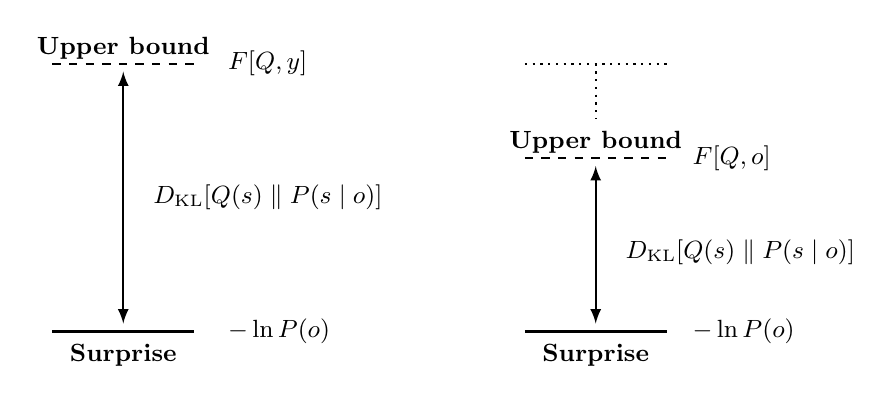
\begin{tikzpicture}[>=latex, thick, font=\small]

% LEFT DIAGRAM

% Upper bound label
\node at (0,4.7) {\textbf{Upper bound}};
\draw[dashed, thick] (-0.9,4.5) -- (0.9,4.5);
\node[anchor=west] at (1.2,4.5) {$F[Q, y]$};

% Vertical Arrow
\draw[<->, thick]  (0,1.2) -- (0,4.4); % extended arrow
\node[anchor=west] at (0.25,2.8) {$D_{\mathrm{KL}}[Q(s) \parallel P(s \mid o)]$};

% Surprise label
\draw[thick] (-0.9,1.1) -- (0.9,1.1);
\node at (0,0.8) {\textbf{Surprise}};
\node[anchor=west] at (1.2,1.1) {$-\ln P(o)$};

% RIGHT DIAGRAM

% Horizontal dotted line matching left dashed line
\draw[dotted, thick] (5.1,4.5) -- (6.9,4.5);

% Vertical Dotted line from above to upper bound
\draw[dotted, thick] (6,4.5) -- (6,3.8);

% Upper bound label
\node at (6,3.5) {\textbf{Upper bound}};
\draw[dashed, thick] (5.1,3.3) -- (6.9,3.3);
\node[anchor=west] at (7.1,3.3) {$F[Q, o]$};

% Vertical Arrow
\draw[<->, thick] (6,1.2) -- (6,3.2);
\node[anchor=west] at (6.25,2.1) {$D_{\mathrm{KL}}[Q(s) \parallel P(s \mid o)]$};

% Surprise label
\draw[thick] (5.1,1.1) -- (6.9,1.1);
\node at (6,0.8) {\textbf{Surprise}};
\node[anchor=west] at (7.1,1.1) {$-\ln P(o)$};

\end{tikzpicture}
\caption{Free energy as an upper bound on surprise. Left: inference as minimization. Right: graphical interpretation.}
\end{figure}